% ============================================================
% Relatório Final — PIP/UFG
% Arial 12pt, espaço 1,5, A4, máx. 15 páginas (excluindo Informações Complementares)
% Compilar: pdflatex relatorio_final_pip.tex
% Fonte: helvet (substituto LaTeX para Arial)
% ============================================================
\documentclass[12pt, a4paper]{article}

% ── Codificação e língua ────────────────────────────────────
\usepackage[utf8]{inputenc}
\usepackage[T1]{fontenc}
\usepackage[brazil]{babel}

% ── Fonte Arial (helvet) ────────────────────────────────────
\usepackage{helvet}
\renewcommand{\familydefault}{\sfdefault}

% ── Margens e espaçamento ───────────────────────────────────
\usepackage[top=1.7cm, bottom=1.6cm, left=2.2cm, right=1.8cm]{geometry}
\usepackage{setspace}
\onehalfspacing

% ── Tabelas e figuras ───────────────────────────────────────
\usepackage{booktabs}
\usepackage{graphicx}
\usepackage{float}
\usepackage{caption}
\usepackage{subcaption}
\captionsetup{font=small, labelfont=bf, skip=4pt, belowskip=2pt}
\captionsetup[sub]{font=small, skip=2pt}
\setlength{\abovecaptionskip}{4pt}
\setlength{\belowcaptionskip}{2pt}
\setlength{\intextsep}{4pt}
\setlength{\textfloatsep}{5pt}
\setlength{\floatsep}{4pt}
\usepackage{array}
\renewcommand{\arraystretch}{0.9}

% ── Matemática ──────────────────────────────────────────────
\usepackage{amsmath}
\usepackage{amssymb}
\setlength{\abovedisplayskip}{4pt}
\setlength{\belowdisplayskip}{4pt}
\setlength{\abovedisplayshortskip}{2pt}
\setlength{\belowdisplayshortskip}{2pt}

% ── Links e metadados ───────────────────────────────────────
\usepackage[hidelinks]{hyperref}
\usepackage{microtype}

% ── Anexos (certificados em PDF) ────────────────────────────
\usepackage{pdfpages}

% ── Código ──────────────────────────────────────────────────
\usepackage{listings}
\lstset{
  basicstyle=\small\ttfamily,
  breaklines=true,
  frame=single,
  columns=flexible,
}

% ── Cabeçalho / rodapé ─────────────────────────────────────
\usepackage{fancyhdr}
\pagestyle{fancy}
\fancyhf{}
\rhead{\small PIP/UFG 2025--2026}
\lhead{\small Yan Santos Leite}
\cfoot{\thepage}
\setlength{\headheight}{14.5pt}      % evita warning "headheight too small" do fancyhdr
\addtolength{\topmargin}{-2.5pt}     % compensa o aumento, mantendo a área de texto
\emergencystretch=2em                % reduz "Overfull \hbox" em parágrafos justificados

% ── Seções sem recuo ────────────────────────────────────────
\setlength{\parindent}{1.25cm}
\setlength{\parskip}{0pt}
\usepackage{titlesec}
\titlespacing*{\section}{0pt}{4pt}{2pt}
\titlespacing*{\subsection}{0pt}{3pt}{1pt}

% ── Título do documento ─────────────────────────────────────
\title{
  \textbf{MÉTODOS MODERNOS PARA PLANEJAMENTO DE TRAJETÓRIA \\ PARA VEÍCULOS AUTÔNOMOS} \\[6pt]
  \large\textit{Desenvolvimento de Framework Adaptivo para Seleção de Algoritmos \\
  de Planejamento de Trajetória em Navegação Autônoma}
}
\author{
  Yan Santos Leite\textsuperscript{1} \and
  Aldo André Diaz Salazar\textsuperscript{2} \\[4pt]
  \small\textsuperscript{1}Estudante, Escola de Engenharia Elétrica, Mecânica e de Computação, UFG \\
  \small leiteyan@discente.ufg.br \\[2pt]
  \small\textsuperscript{2}Orientador, Instituto de Informática, UFG \\
  \small aldo.diaz@ufg.br
}
\date{Agosto/2026, Relatório final}

% ============================================================
\begin{document}

\vspace{-1.5cm}
\maketitle
\vspace{-1.2cm}
\thispagestyle{fancy}

% ── Resumo ──────────────────────────────────────────────────
\begin{abstract}
Todo robô autônomo precisa decidir por onde passar. Algoritmos clássicos como o A* resolvem essa
decisão em milissegundos num corredor vazio, mas seu custo cresce à medida que obstáculos se
acumulam ao redor; políticas aprendidas pagam sempre o mesmo preço, qualquer que seja a densidade,
e desperdiçam esse preço quando o caminho já está livre. A escolha entre os dois costuma ser
feita uma vez, na prancheta, e nunca mais revista. Um sistema assim fica mal ajustado a ambientes
heterogêneos, em que a densidade de obstáculos muda ao longo do próprio percurso.

Este trabalho sustenta que escolher o planejador durante a navegação, e não antes dela, mantém o
desempenho do melhor planejador fixo por uma fração pequena do seu custo computacional
(Seção~\ref{sec:h1_real}). A hipótese inicial era mais ambiciosa: superar qualquer escolha fixa
em taxa de acerto. Ela se sustentou apenas sob planejadores calibrados por modelo estatístico
(Seção~\ref{sec:validacao_fase1}), e caiu no teste com planejadores reais.

A contribuição central é o $\rho$-\textit{criterion}, onde $\rho$ é a densidade local de
obstáculos ao redor do robô. O critério mede essa densidade e escolhe, em tempo real, entre A* em
espaços abertos e uma política de \textit{Behavior Cloning} (BC) em regiões congestionadas, onde
a política aprendida lida melhor com geometrias difíceis a custo constante. Uma varredura de
1.500 cenários, cobrindo densidades de $0{,}10$ a $0{,}60$, localizou o ponto de troca em
$\rho^* = 0{,}30$.

Na Fase~1, sobre modelos calibrados, o critério alcançou 85,3\% de taxa de sucesso contra 76\% do
melhor método fixo. O benchmark dos algoritmos clássicos justificou a escolha do A* como
componente: o Floyd-Warshall consome 48,3~s e 22,9~MB num grid $30{\times}30$, inviável em tempo
real. A Fase~2 integrou ROS2~Humble, Gazebo~Classic e TurtleBot3~Waffle; a infraestrutura ficou
implementada e depurada, mas a validação quantitativa de navegação real não foi concluída nesta
IC, lacuna declarada como limitação central.

Revalidamos H1 com A* e BC reais no gêmeo 2D, o ambiente de simulação leve descrito na
Seção~\ref{sec:integracao}, sobre 1.500 \textit{trials} pareados. A motivação original não
sobreviveu: o A* real acertou 88,2\% contra 84,3\% do critério adaptivo, diferença significativa
pelo teste de McNemar, que compara dois métodos pareados sobre os mesmos casos
($p = 5{,}4 \times 10^{-5}$). Já a motivação por custo saiu reforçada, com razão de
$\sim$656$\times$ medida no mesmo ambiente contra $\sim$10$\times$ estimado antes. H1 passa
então a ser um argumento de custo computacional: o ganho do $\rho$-criterion está em sustentar
desempenho competitivo por uma fração do custo do melhor planejador fixo, sem necessariamente
superá-lo em sucesso bruto.

\vspace{4pt}
\noindent Palavras-chave: planejamento de trajetória; navegação autônoma; robótica
móvel; seleção de algoritmos (\textit{algorithm selection}); aprendizado por imitação
(\textit{behavior cloning}); aprendizado por reforço profundo; ROS2; Nav2; sistemas híbridos de
planejamento; densidade de obstáculos.
\end{abstract}


% ============================================================
\section{Apresentação: Introdução, Justificativa e Trabalhos Relacionados}

Nenhum planejador único é universalmente ótimo em ambientes heterogêneos. Num corredor aberto, o
A* encontra caminhos ótimos em milissegundos; num depósito densamente obstruído ou num cruzamento
urbano, políticas aprendidas reagem ao ambiente local sem depender de um mapa completo. A
densidade de obstáculos ao redor do robô prediz qual dos dois regimes vale a pena pagar, porque
mede exatamente a dificuldade geométrica que separa um caso do outro. Decidir qual comportamento
adotar a cada instante, e não apenas como executá-lo, é o núcleo deste trabalho.

O problema tem nome na literatura: \textit{algorithm selection} \cite{Rice1976}, escolher para
cada instância, com base em características observáveis dela, qual entre vários algoritmos
executar. Quatro trabalhos recentes atacam a mesma combinação de aprendizado e planejamento em
navegação robótica. Nenhum deles comuta entre dois planejadores completos a partir de uma leitura
contínua do ambiente.

Xu et al.\ \cite{Xu2020} (APPLR) usam aprendizado por reforço para ajustar em tempo real os
parâmetros internos de um planejador clássico já existente, como o raio de busca ou o peso de
custo. O aprendizado ali serve para calibrar um planejador, jamais para escolher entre dois.
Damanik et al.\
\cite{Damanik2024} (LiCS), vencedores do BARN Challenge na ICRA 2024, apostam no extremo oposto ao
deste trabalho: treinam uma única política de imitação forte o bastante para cobrir sozinha
ambientes muito diferentes, dispensando qualquer comutação. Já Kolomeytsev e Golembiovsky
\cite{Kolomeytsev2025} (HMP-DRL) combinam um planejador global em grafo, que traça a rota macro,
com uma política local que ajusta o movimento fino; o planejador global, porém, nunca se desliga,
mesmo quando o trecho não exige seu custo.

Os dois trabalhos mais próximos deste de fato comutam entre planejadores completos. Sharma et
al.\ \cite{Sharma2024} alternam entre DWA e uma política de RL por uma regra heurística fixa de
\textit{clearance detection}, que verifica se waypoints do plano global estão bloqueados por
leituras consecutivas de LiDAR. Não há camada de decisão aprendida, e o gatilho é reativo: só
dispara depois que o obstáculo já bloqueou o caminho. Dey et al.\ \cite{Dey2023} treinam um
planejador de alto nível que decide, a cada passo, se confia num planejador clássico ou numa
política neural, aprendendo esse gatilho fim a fim a partir da interação do robô com o ambiente.

Em relação a esses dois trabalhos, a contribuição deste está em usar uma variável de contexto
explícita e de custo desprezível: a densidade local de obstáculos $\rho$
(Seção~\ref{sec:criterio_adaptivo}). Diferente do gatilho reativo de Sharma et al.\ e do gatilho
aprendido de Dey et al., a densidade $\rho$ antecipa a necessidade de comutação antes que o
planejador clássico chegue a travar, sem exigir que esse gatilho seja, ele próprio, uma política
treinada à parte.

Daí a pergunta que este trabalho investiga: a seleção adaptiva de planejador, guiada pela
densidade local de obstáculos, consegue manter o desempenho do melhor planejador fixo pagando
apenas uma fração do seu custo computacional em ambientes heterogêneos?

A pergunta se desdobra em três hipóteses verificáveis:

\begin{itemize}
  \item[] \textbf{H1 (desempenho):} o critério adaptivo alcança taxa de sucesso próxima à do
    melhor método fixo, não necessariamente superior a ela, pagando uma fração pequena do seu
    custo de decisão, em ambientes de densidade variável.
  \item[] \textbf{H2 (qualidade do limiar):} o limiar $\rho^*{=}0{,}30$ acerta o ponto de troca
    entre o planejador clássico e o de aprendizado, aproximando-se de um seletor ideal: diferença
    média de até 5\%, e de até 10\% no pior caso.
  \item[] \textbf{H3 (realizabilidade):} o framework é realizável em um \textit{stack} robótico
    padrão da indústria (ROS2/Nav2/Gazebo), sem exigir modificação dos planejadores subjacentes.
\end{itemize}

Este trabalho foi desenvolvido pelo autor como discente do Programa de Iniciação à Pesquisa da
UFG (PIP/UFG), modalidade IC, no período 01/09/2025--31/08/2026, vinculado ao projeto
PI08078-2024. Ele está alinhado ao Plano de Trabalho, que prevê a comparação entre métodos
clássicos e modernos por métricas de tempo e memória; ao Parecer do Consultor SIGAA
(13/06/2025), que exige implementações otimizadas dos algoritmos clássicos; e ao Relatório
Parcial (aprovado em 01/04/2026), do qual o $\rho$-criterion é evolução direta (Objetivo~4).

O objetivo geral definido no Plano de Trabalho (PI08078-2024) é investigar, implementar e
comparar métodos clássicos e modernos de planejamento de trajetória para veículos autônomos em
ambientes urbanos, com foco em eficiência, adaptabilidade e aplicabilidade simulacional na
navegação robótica. Desse objetivo geral decorrem cinco objetivos específicos: (1)~implementar os
algoritmos clássicos Dijkstra, A*, Floyd-Warshall e Johnson; (2)~avaliar seu desempenho em
cenários estáticos, dinâmicos e com obstáculos; (3)~identificar e testar abordagens de
aprendizado por reforço profundo; (4)~comparar métodos clássicos e modernos quanto a tempo de
execução e eficiência computacional; e (5)~empregar Python, C++, ROS e Gazebo como ferramental.
A cobertura de cada um desses objetivos, com status honesto sobre o que foi ou não cumprido, é
apresentada na Conclusão.

% ============================================================
\section{Metodologia: Algoritmos Clássicos, Critério Adaptivo \texorpdfstring{$\rho$}{rho}, Regret Teórico e Protocolo}
\label{sec:criterio_adaptivo}

Os quatro algoritmos clássicos foram implementados em Python puro, usando estruturas de dados
otimizadas descritas em \cite{Cormen2022}. Essa escolha responde diretamente à observação do
Consultor SIGAA (13/06/2025) de que a comparação deve envolver implementações otimizadas, não
apenas didáticas.

Cada algoritmo usa a estrutura de dados adequada à sua complexidade ótima: Dijkstra e A*
\cite{Hart1968} utilizam \texttt{heapq}, um heap binário mínimo, garantindo $O(V \log V + E)$ na
prática; Floyd-Warshall usa matriz densa, com custo $O(V^3)$ em tempo e $O(V^2)$ em memória;
Johnson usa lista de adjacências com rebalanceamento por Bellman-Ford, custo
$O(V \cdot E \cdot \log V)$, suportando pesos negativos. Os quatro operam sobre grafos
construídos por \texttt{grid\_to\_graph()}, com conectividade 4-direcional. Já o A* usado em
tempo de execução pelo framework real não é essa implementação didática: é o Nav2/SmacPlanner2D
\cite{Macenski2022}, uma implementação em C++ da comunidade ROS2 usada em produção, o que reforça
o caráter da comparação com implementações de qualidade industrial.

A densidade local não apenas se correlaciona com o \textit{trade-off} entre os dois
planejadores: ela estrutura mecanicamente essa escolha. Cada
obstáculo próximo obriga o A* a expandir mais nós e aumenta o fator de ramificação da busca,
enquanto o custo de decisão de uma política aprendida ignora completamente esse crescimento
(Seção~\ref{sec:benchmark_classicos}). Variáveis candidatas como distância ao \textit{goal},
velocidade ou tipo de obstáculo descrevem o estado do robô ou da tarefa, não a dificuldade
geométrica que motiva a troca. E essa dificuldade muda de metro em metro, conforme o robô cruza
regiões abertas e congestionadas da mesma arena, o que exige medi-la localmente.

A comutação usa um corte binário em vez de misturar as duas saídas, por uma restrição de tempo
real. Uma fusão suave exigiria arbitrar entre os planejadores
a cada passo de controle, calculando um peso e executando ambos parcialmente, o que não cabe na
taxa do laço. Ela também trocaria uma garantia de regret limpa (Seção~\ref{sec:regret}) por um
peso contínuo sem alvo claro de calibração. O corte binário é, portanto, um ponto de projeto
deliberado, revisitado na Conclusão.

A densidade local de obstáculos é calculada em uma janela $w = 2{,}0$~m (quadrada, centrada na
pose atual do robô) sobre a costmap de ocupação:

\begin{equation}
  \rho(p, w) = \frac{\lvert\{c \in W(p,w) : \mathrm{occ}(c) \geq 65\}\rvert}{\lvert W(p,w)\rvert}
\end{equation}

O limiar de ocupação $65$ é o \textit{default} do Nav2 para células consideradas obstáculo
(\texttt{occ\_threshold}, \texttt{density\_estimator.py}), não um valor ajustado neste trabalho;
células desconhecidas ($\mathrm{occ}=-1$) são tratadas como ocupadas, por conservadorismo de
segurança.

A política de seleção é:

\begin{equation}
  \pi(\rho) =
  \begin{cases}
    \text{A*} \; (\text{Nav2 SmacPlanner2D}) & \text{se } \rho < 0{,}30 \\
    \text{BC} \; (\text{Behavior Cloning}) & \text{se } \rho \geq 0{,}30
  \end{cases}
\end{equation}

O limiar $\rho^* = 0{,}30$ foi determinado por validação experimental com 1.500 trials.
\label{sec:regret}

Adotamos o vocabulário de \textit{algorithm selection} \cite{Rice1976} para medir a qualidade do
critério: o VBS (\textit{Virtual Best Solver}) é o seletor ideal, o oráculo que, para
cada instância do problema, conhece de antemão qual planejador teria sucesso e sempre o escolhe;
o SBS (\textit{Single Best Solver}) é o melhor planejador único fixo em todas as
instâncias (o A* na Seção~\ref{sec:h1_real}). O regret do critério
adaptivo $\pi$ é a distância ao VBS:

\begin{equation}
  \mathrm{Regret}(\pi) = \mathbb{E}[R_{\mathrm{VBS}}] - \mathbb{E}[R_\pi]
\end{equation}

Quanto menor o regret, mais perto o critério está do VBS. Um critério de seleção só se justifica
como contribuição se aproximar o VBS mais do que o SBS sozinho já aproxima; caso contrário,
bastaria usar sempre o melhor planejador fixo. Nos experimentos calibrados (Monte Carlo), o
$\rho$-criterion cumpre esse requisito com folga: fica, em média, a apenas $2{,}9\%$ do VBS, e a
$6{,}7\%$ no pior caso.

Na Fase~2, voltada à realizabilidade em um \textit{stack} robótico real (H3), o sistema integra
ROS2 Humble, Gazebo Classic (v11), TurtleBot3 Waffle, Nav2 SmacPlanner2D e SAC
\cite{Haarnoja2018} via Stable-Baselines3 \cite{Raffin2021}. O ambiente \textit{gym} customizado
recebe observações de 29 dimensões: 24 raios LIDAR subamostrados de 360°, distância e ângulo ao
\textit{goal} em coordenadas polares, \textit{yaw} relativo, e a ação anterior do robô
(velocidades linear e angular normalizadas). Incluir a ação anterior remedia a observabilidade
parcial do problema (um POMDP), dando ao agente uma memória de curto prazo do próprio
movimento. As ações de saída controlam a velocidade linear e a angular, ambas normalizadas no
intervalo $[-1, 1]$.

Já o benchmark dos algoritmos clássicos segue um protocolo à parte, independente do ROS2/Gazebo.
Cada algoritmo foi testado em grids de tamanho crescente, de $10\times10$ a $50\times50$, com
densidade fixa de obstáculos em 25\% e 30 \textit{trials} por configuração de tamanho. Em cada
\textit{trial}, três grandezas foram medidas: o tempo de execução
(\texttt{timeit.perf\_counter()}), a memória de pico
(\texttt{tracemalloc.get\_traced\_memory()}) e a alcançabilidade, isto é, a fração de trials com
origem-destino conectados). Todos os experimentos de tempo de execução e custo computacional
deste relatório, o benchmark dos clássicos, o custo A*/BC no gêmeo 2D e a aceleração do 2D em
relação ao Gazebo, rodam na mesma CPU única: um Intel Core i5-1235U, com 12 \textit{threads}, sem
GPU e 23~GB de RAM; qualquer comparação de tempo absoluto entre este trabalho e outros deve
considerar essa configuração.

% ============================================================
\section{Resultados e Discussão}

\subsection{Benchmark dos Algoritmos Clássicos e Validação do Critério \texorpdfstring{$\rho$}{rho}: Fase 1 (Monte Carlo)}
\label{sec:benchmark_classicos}
\label{sec:validacao_fase1}

\begin{table}[H]
  \centering
  \caption{Tempo de execução (ms) e memória de pico (KB), média por algoritmo e grid}
  \label{tab:tempo_memoria}
  \begin{tabular}{lrrrrrrrr}
    \toprule
    & \multicolumn{3}{c}{\textbf{Tempo (ms)}} & \multicolumn{3}{c}{\textbf{Memória (KB)}} \\
    \textbf{Algoritmo} & 10² & 30² & 50² & 10² & 30² & 50² \\
    \midrule
    Dijkstra        & 0,101 & 0,892 & 2,38     & 3,5 & 29,2 & 79,4 \\
    A*              & 0,101 & 0,950 & 2,90     & 5,8 & 49,3 & 190,1 \\
    Floyd-Warshall  & 38,3  & 48.339 & inviável & 283 & 23.472 & --- \\
    Johnson         & 9,4   & 983   & inviável  & 617 & 59.018 & --- \\
    \bottomrule
  \end{tabular}
\end{table}

\noindent\small\textit{Dados: junho/2026; semente 42; densidade 25\%; Python 3.10 (hardware na
Seção~\ref{sec:regret}). Grid $N{\times}N$; coluna 20² omitida por concisão.}

Dijkstra e A* crescem linearmente, com complexidade $O(V \log V)$ na prática. Floyd-Warshall
cresce cubicamente, saltando $\approx 92\times$ de 10$\times$10 para 20$\times$20, e deixa de ser
viável a partir de 50$\times$50. Entre os quatro, apenas o A* combina escalabilidade com
direcionamento ao objetivo, e por isso entra no framework como componente clássico.

Validado o A*, a Fase~1 avalia o critério adaptivo completo em 1.500 \textit{trials} de simulação
2D sob protocolo Monte Carlo: cada \textit{trial} sorteia um cenário, com posição do robô, do
objetivo e densidade de obstáculos, e a taxa de sucesso é a frequência de acerto ao longo das
repetições. O protocolo desta fase é \textit{calibrado}, com uma ressalva importante: os métodos
comparados não são reimplementações originais, e sim proxies estatísticos que reproduzem as taxas
de sucesso reportadas nos respectivos artigos.

\textbf{Como o limiar foi determinado, e por que $\rho^*{=}0{,}30$ é mantido.} Testamos limiares
candidatos de 0,10 a 0,60 (500 cenários por limiar, densidades sorteadas nesse intervalo, regra
``A* abaixo do limiar, política aprendida acima''), sob planejadores mock e, depois, sob A* e BC
reais (\texttt{sweep\_threshold\_real.py}, $n{=}1.500$, \textit{split} treino/teste de
750/750 para separar calibração de avaliação). Em nenhum dos dois protocolos o regret mínimo
coincide com $\rho^*{=}0{,}30$: no mock, o mínimo é em $\tau{=}0{,}20$ ($0{,}60\%$, contra
$2{,}92\%$ em $\tau{=}0{,}30$); no real, o regret decai estritamente até o extremo testado, sem
mínimo interno ($8{,}4\%$ em $\tau{=}0{,}30$ contra $7{,}5\%$ em $\tau{=}0{,}60$, uma diferença de
apenas $0{,}9$ pontos percentuais).

O que sustenta $\rho^*{=}0{,}30$ é o custo, não o regret mínimo. Nesse ponto, o tempo do A* já
subiu de 16~ms para 115~ms, enquanto a política aprendida se mantém em $\approx$12~ms, e essa
divergência justifica cortar antes do que o cruzamento de sucesso puro sugeriria. Adotar
$\tau{=}0{,}60$ como novo limiar também não se justificaria: a curva é achatada nessa região,
com apenas $0{,}7$ pontos percentuais de diferença de sucesso entre $\tau{=}0{,}40$ e
$\tau{=}0{,}60$, e $\rho^*{=}0{,}30$ já está em uso em toda a Fase~2 e na
Seção~\ref{sec:h1_real}. Uma recalibração em cascata custaria mais do que essa margem vale.
Mantemos $\rho^*{=}0{,}30$ por continuidade entre ambientes e por custo, com a ressalva explícita
de que a escolha sacrifica cerca de $1$ ponto percentual de regret frente ao melhor ponto testado
em cada protocolo (ver Limitações).

\begin{table}[H]
  \centering
  \caption{Comparação de métodos: Fase 1 (simulação Monte Carlo calibrada)}
  \label{tab:fase1}
  \begin{tabular}{llr}
    \toprule
    \textbf{Método} & \textbf{Tipo} & \textbf{Taxa de sucesso} \\
    \midrule
    Framework adaptivo $\rho$-criterion & Mock calibrado (este trabalho) & 85,3\% \\
    PPO fixo                            & Mock calibrado (este trabalho) & 76,0\% \\
    RRT* fixo                           & Mock calibrado (este trabalho) & 48,0\% \\
    Comutação aleatória (ablação)       & Mock calibrado (este trabalho) & 65,4\% \\
    \bottomrule
  \end{tabular}
\end{table}

O framework adaptivo (Tabela~\ref{tab:fase1}) supera tanto os métodos fixos quanto a ablação de
comutação aleatória, que atinge 65,4\% sorteando a decisão em vez de consultar $\rho$, sob a
mesma regra de comutação e as mesmas densidades, em protocolo de maior escala ($n{=}2.500$). O
contraste isola a fonte do ganho: comutar por densidade, e não meramente alternar entre
planejadores. Contra o melhor método fixo, o PPO com 76,0\%, um teste de proporções unilateral
confirma a diferença ($z = 2{,}05$, $p = 0{,}020$, $\alpha = 0{,}05$, $n = 150$ trials por
método no subconjunto pareado dos 1.500 da varredura), com tamanho de efeito Cohen's
$h = 0{,}24$. O regret médio em relação ao seletor ideal fica em 2,9\%, com 6,7\% no pior caso,
dentro do limite de 10\% previsto por H2.

\textit{Nota de honestidade metodológica.} A tabela mede a auto-consistência do mecanismo de
comutação sob o protocolo mock original, com o limiar fixo em $\rho^*{=}0{,}30$ ao longo de todo
o experimento. Trate-a como estudo de viabilidade do critério, não como validação final de
desempenho de navegação.


\subsection{Integração ROS2/Gazebo, Validação no Gêmeo 2D, Revalidação de H1 e Extensão Multi-Agente}
\label{sec:integracao}

A infraestrutura ROS2 Humble + Gazebo Classic~(v11) + TurtleBot3 Waffle + Nav2 SmacPlanner2D +
SAC \cite{Haarnoja2018} via Stable-Baselines3 \cite{Raffin2021} está integrada e operacional, com
observação de 29 dimensões (Seção~\ref{sec:criterio_adaptivo}) e reprodutibilidade via Docker
Compose (seed=42, \texttt{models/best\_model.zip}), validando H3.\footnote{Hiperparâmetros do
SAC: \texttt{ent\_coef=0.1} fixo (\texttt{auto}~+~gSDE colapsava a exploração), gSDE,
\texttt{gradient\_steps=1}, buffer 1M, episódios de 200 passos, currículo de distância inicial
1,0~m crescendo 0,5~m a cada 60\% de sucesso.} A função de recompensa segue a formulação
minimalista consolidada na literatura de navegação DRL com LIDAR \cite{Cimurs2022, deJesus2021}:

\begin{equation}
  r(s,a) =
  \begin{cases}
    +100 & \text{goal atingido} \\
    -100 + R_{\mathrm{prox}} & \text{colisão} \\
    R_{\mathrm{surv}} + \max(0,\; R_{\mathrm{app}}(d_{t-1} - d_t)) & \text{caso contrário}
  \end{cases}
\end{equation}

\noindent onde $R_{\mathrm{surv}}{=}0{,}1$ é o bônus de sobrevivência e
$R_{\mathrm{prox}}{=}1 - d_t/d_{t-1}$ o crédito de progresso, o que mantém a recompensa por passo
sempre $\geq 0$. Versões iniciais penalizavam obstáculo a cada passo, e a soma dessas penalidades
superava a penalidade terminal de colisão: colidir cedo virava a estratégia racional. O
\textit{suicidal agent} aparecia na queda de $\mathrm{ep\_len\_mean}$ de ${\sim}55$ para
${\sim}8$ passos. A correção, seguindo Cimurs et al.\ (2022), elimina a penalidade por passo.

Iterar reward diretamente no Gazebo é lento demais para ser prático. Por isso implementamos um
ambiente 2D leve (\texttt{eval/env2d/}) com raycasting vetorizado em NumPy, $851\times$ mais
rápido que o Gazebo Classic, reproduzindo a mesma cinemática unicycle, a mesma observação de 29
dimensões e a mesma estrutura de recompensa do ambiente ROS2. Nele o SAC converge a 90\% de taxa
de sucesso em $\leq$14.000 passos, ou $\leq$3,3 minutos, no mundo esparso, com reprodução em 3
seeds independentes. Foi esse ciclo curto que expôs um desalinhamento no bônus de aproximação
(\texttt{R\_APPROACH}) até então invisível: corrigido, o treino no Gazebo passou a apresentar
episódios estáveis e crescentes (Fig.~\ref{fig:2d_heatmap}).

\begin{figure}[H]
  \centering
  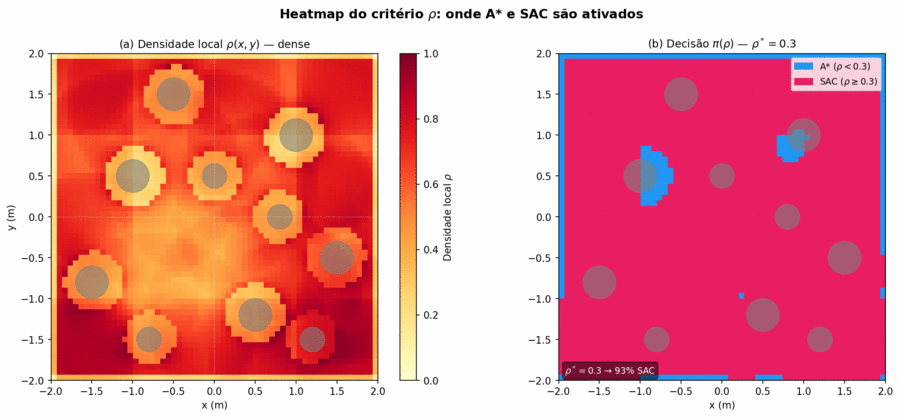
\includegraphics[width=0.48\textwidth]{figs/2d/fig_2d_heatmap_dense.png}
  \caption{Mapa de decisão $\rho$-criterion no ambiente denso: azul ($\rho{<}0{,}30$) usa A*,
           vermelho usa BC.}
  \label{fig:2d_heatmap}
\end{figure}


O modelo \texttt{sac\_2d\_best} foi treinado apenas no mundo \texttt{sparse} ($\rho{=}0{,}05$),
o que permite diagnosticar sua generalização por densidade. Avaliá-lo em 100 episódios por densidade, sem
novo treinamento, mede o quanto ele generaliza para fora dessa distribuição
(Figura~\ref{fig:ic_degradation}). A queda é acentuada: 91\% de sucesso no esparso, 59\% no denso,
40\% no muito denso. Colisão domina os modos de falha, à frente do \textit{timeout}, o que indica
que o agente encontra obstáculos antes de ter tempo de explorar o espaço. O próximo passo de treinamento
decorre daí: um currículo multi-densidade (sparse $\to$ dense $\to$ very\_dense), previsto para
quando o treino no Gazebo liberar recursos computacionais.

\begin{figure}[H]
  \centering
  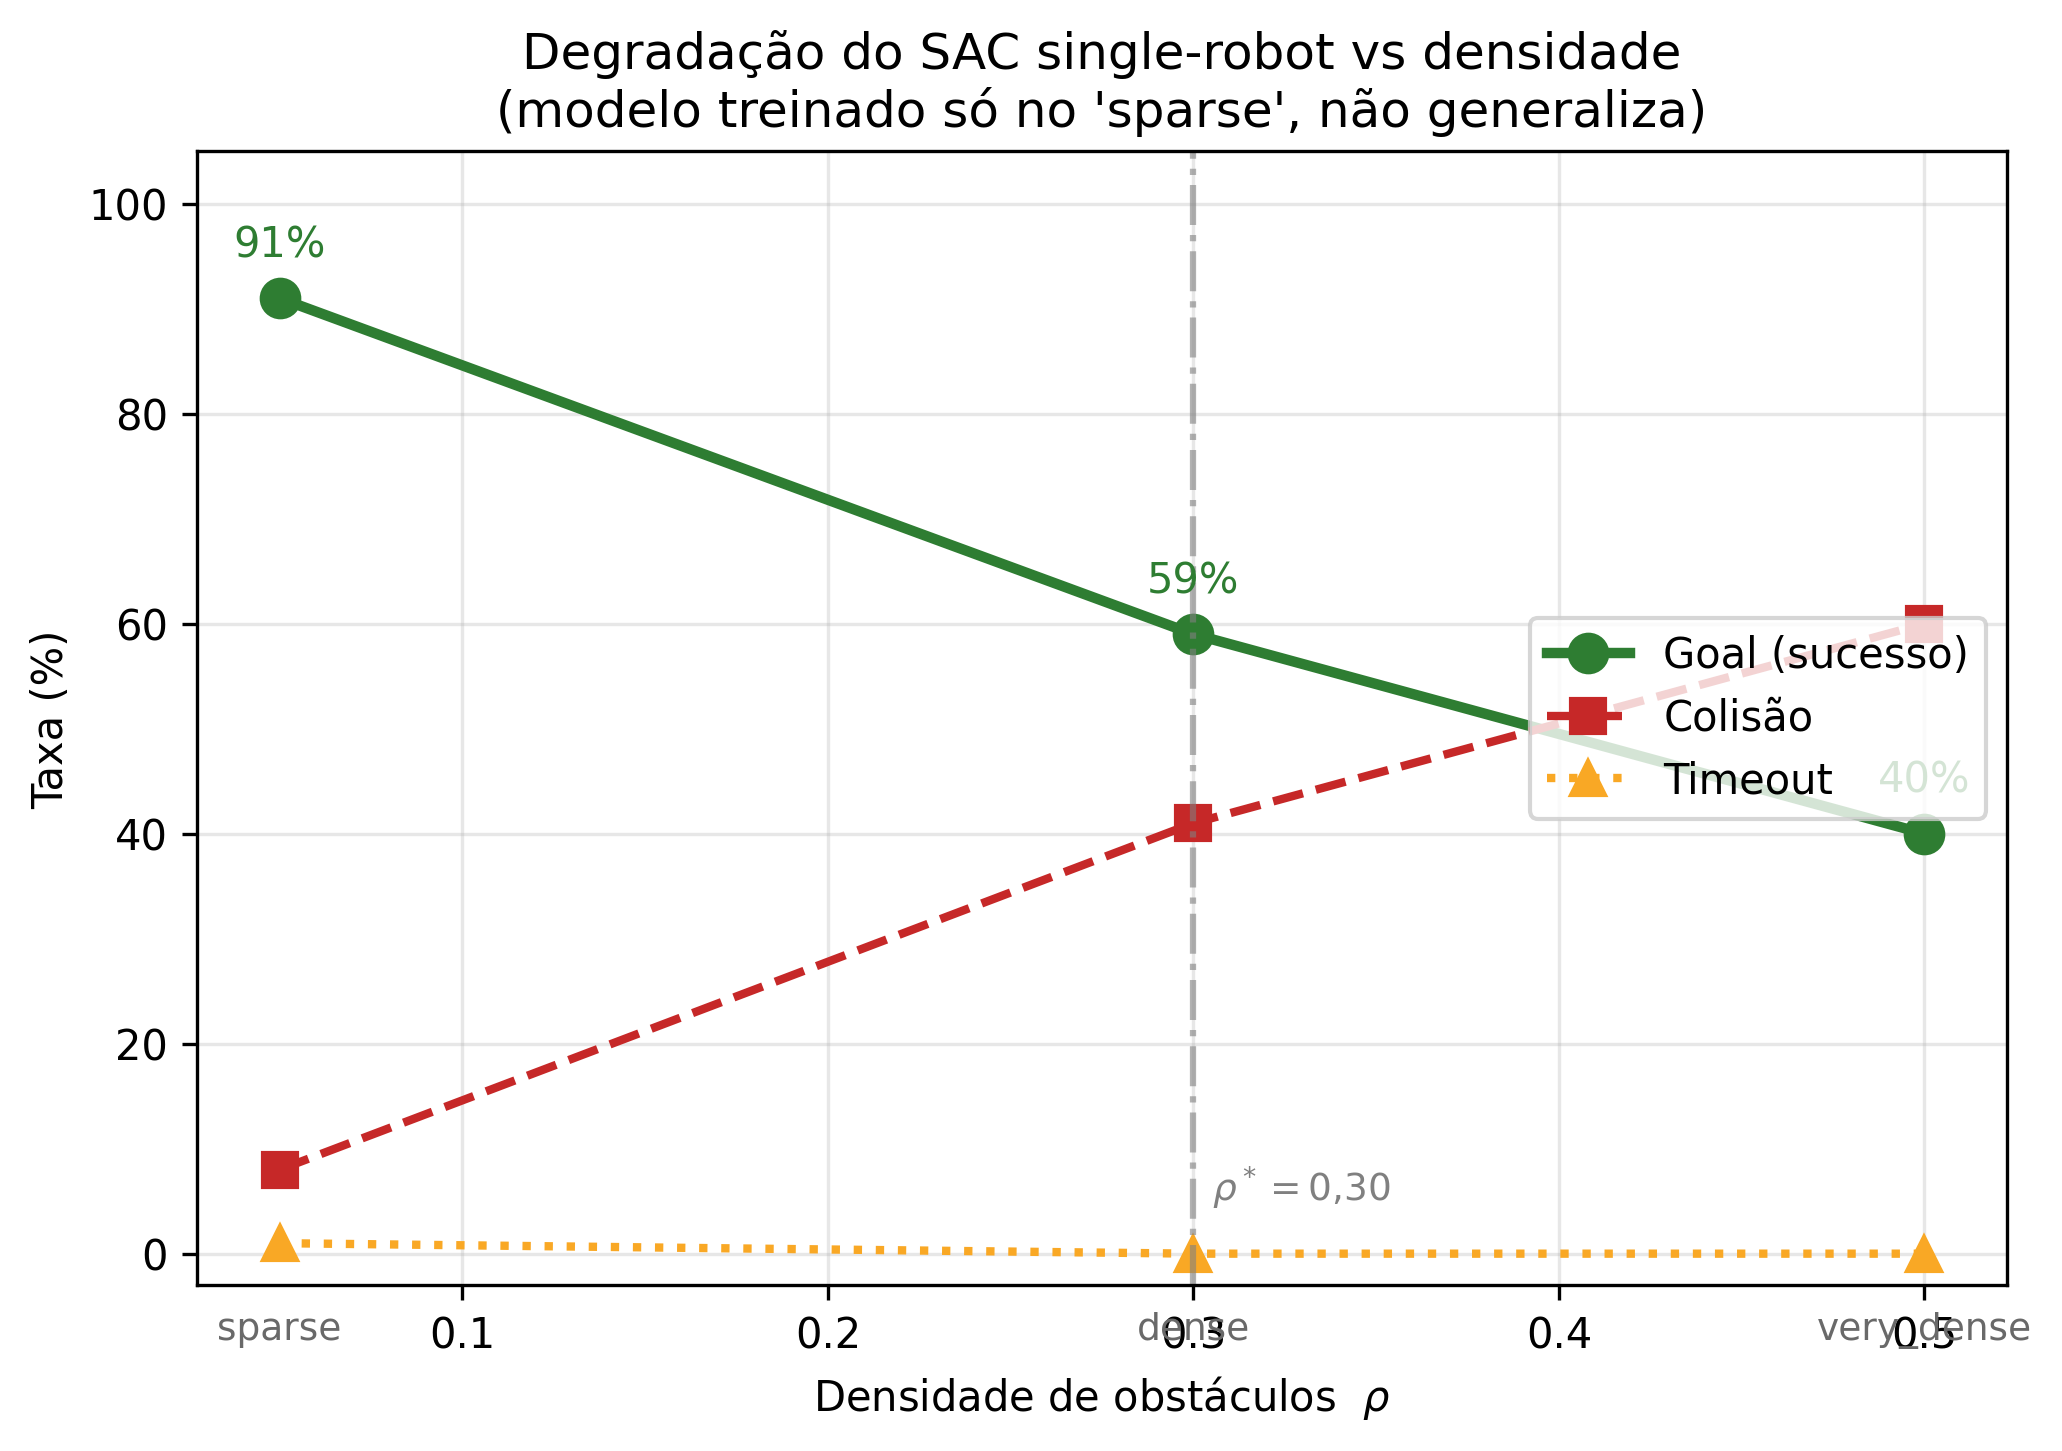
\includegraphics[width=0.55\textwidth]{figs/2d/fig_2d_degradation_singlerobot.png}
  \caption{Degradação do SAC (treinado só em \textit{sparse}) por densidade $\rho$.}
  \label{fig:ic_degradation}
\end{figure}

Um bug de infraestrutura, detalhado na Limitação~1, impediu a conclusão da validação quantitativa
em Gazebo dentro desta IC. A Fase~2 encerrou-se, então, no nível de infraestrutura: pipeline,
ambiente Gym, integração ROS2$\leftrightarrow$Gazebo e mecanismos de resiliência (checkpoint,
replay buffer, auto-resume) ficaram funcionais. A lacuna restringe-se à validação quantitativa de
navegação e não alcança a arquitetura, o que confirma a parte de H3 relativa à realizabilidade e
credencia o ambiente 2D como proxy para depurar recompensa antes do ciclo lento da simulação
física. Bugs menores identificados ao longo da integração ROS2/Gazebo estão documentados no
repositório.

O \textit{Behavior Cloning} (BC), imitação supervisionada de um controlador de campo potencial,
reforça esse diagnóstico: atingiu 98\% de sucesso em cerca de 2 minutos de treino no mesmo
ambiente, o melhor resultado quantitativo de navegação desta IC
(Figura~\ref{fig:ic_bc_trajectory}). Se um segundo paradigma aprende bem onde o SAC tropeça, a
limitação está na infraestrutura de treino, não no critério $\rho$.

\begin{figure}[H]
  \centering
  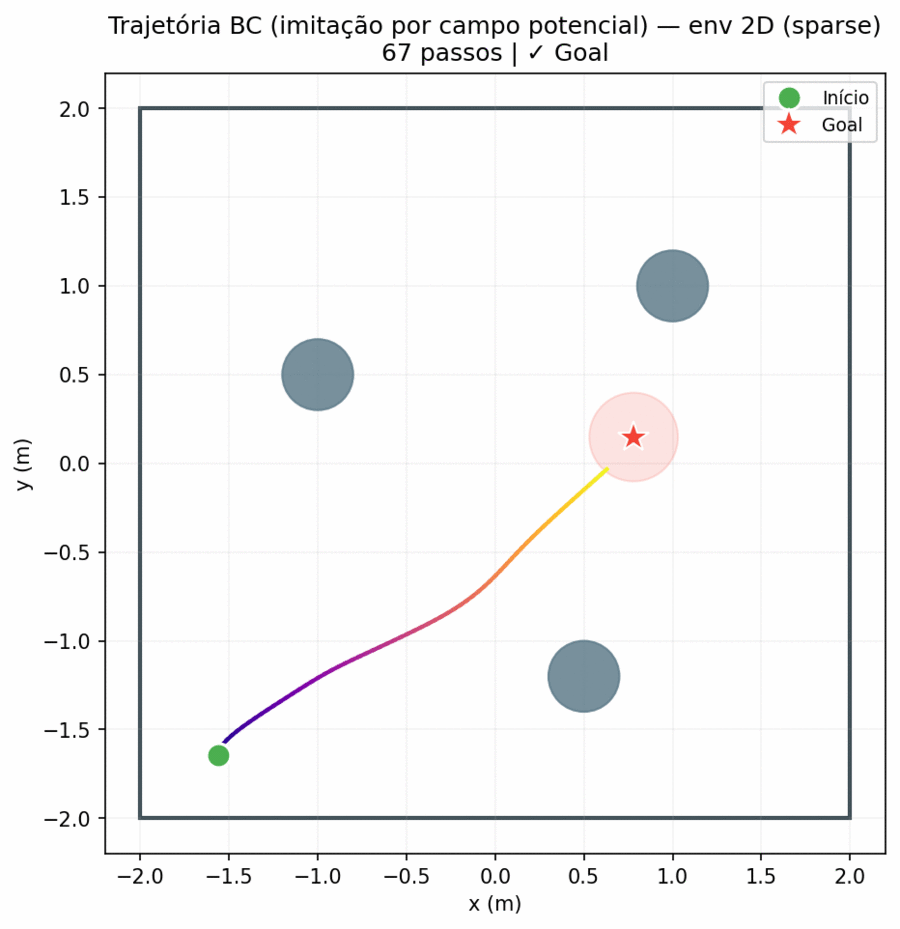
\includegraphics[width=0.5\textwidth]{figs/2d/fig_2d_bc_trajectory_sparse.png}
  \caption{Trajetória do agente BC (\textit{sparse}), gradiente temporal até o goal.}
  \label{fig:ic_bc_trajectory}
\end{figure}

\label{sec:h1_real}

Para reduzir a dependência de planejadores mock (Seção~\ref{sec:validacao_fase1}) sem precisar
do Gazebo, implementamos um A* real (busca em grade 8-conectada, heap binário, heurística
octile, mesma estrutura de dados exigida pelo parecer do consultor SIGAA) dentro do gêmeo 2D,
substituindo a política de linha reta que estava incorretamente rotulada como ``A*'' nas
comparações multiagente anteriores. Revalidamos H1 com A* real e BC real (treinado
especificamente por densidade, \textit{sparse}/\textit{dense}/\textit{very\_dense}) num
protocolo de 1.500 trials com pool misto de densidades, pareado por trial (mesma estrutura de
regret do Monte Carlo original: regret = sucesso do oracle $-$ sucesso do método, oracle =
melhor entre A* e BC em cada trial individual). O número de trials iguala a escala do Monte
Carlo original da Seção~\ref{sec:validacao_fase1}, permitindo comparação direta de poder
estatístico entre as duas validações; um piloto inicial com 500 trials já mostrava o mesmo
padrão qualitativo, usado para validar o protocolo antes de escalar.

\begin{figure}[H]
  \centering
  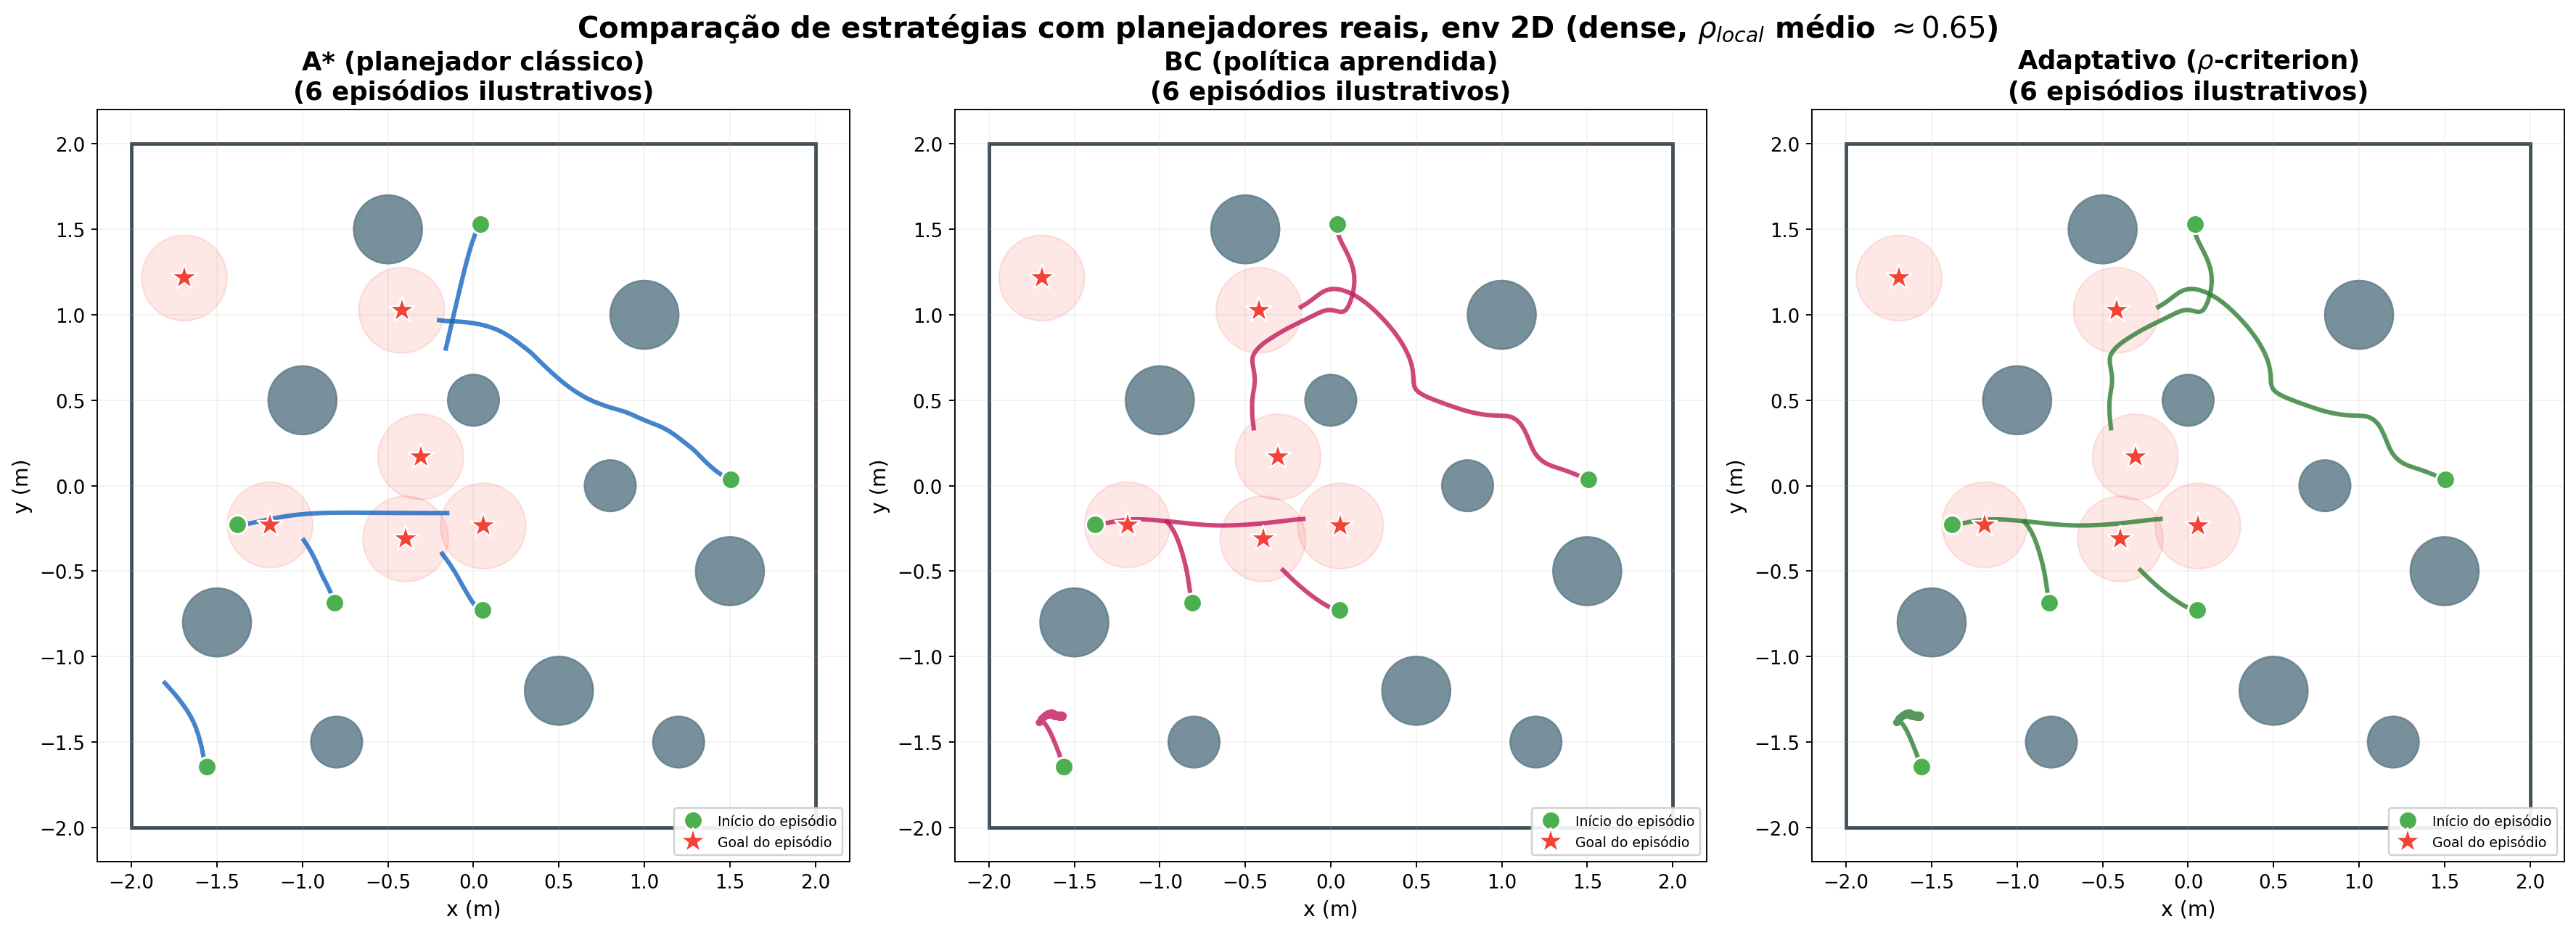
\includegraphics[width=0.92\textwidth]{figs/2d/fig_2d_compare_dense.png}
  \caption{Trajetórias reais no mesmo ambiente denso, para os mesmos pares de início/destino:
           A* (busca em grafo), BC (\textit{Behavior Cloning}) e o $\rho$-criterion adaptativo.
           Amostra ilustrativa; a taxa de sucesso real (n=1.500) está na Figura~\ref{fig:h1_real_validation}.}
  \label{fig:compare_dense}
\end{figure}

\textbf{Achado principal.} Com planejadores reais, a motivação por taxa de sucesso não se
sustenta. O A* venceu em praticamente todo o espectro de densidade testado, com 88,2\% de sucesso
pareado contra 84,3\% do BC e os mesmos 84,3\% do $\rho$-criterion em $\rho^*{=}0{,}30$. O regret
real contra o VBS chega a 8,7\%, bem acima dos 2,9\% observados sob os planejadores mock.

A coincidência entre o critério e o BC isolado, até a primeira casa decimal, tem explicação
direta na composição da amostra. Dos 1.500 trials do pool misto, $87{,}5\%$ têm
$\rho_0 \geq 0{,}30$ e vão para o BC, contra apenas $12{,}5\%$ roteados ao A*. Dominado por
cenários densos, o agregado do critério aproxima-se do de uma política ``sempre BC'', ainda que o
A* vença com folga a fatia esparsa que o critério de fato lhe destina.

A diferença entre A* e $\rho$-criterion é estatisticamente significativa. Os dois métodos
discordaram em 202 dos 1.500 trials, e o A* levou 130 dessas discordâncias contra 72 do
adaptivo (McNemar exato, $p{=}5{,}4{\times}10^{-5}$). Neste testbed não existe faixa de densidade
em que o BC supere o A* em taxa de sucesso.

\textbf{Chattering e correção por histerese.} Um limiar único, sem zona morta, é suscetível a
oscilação de decisão perto de $\rho^*{=}0{,}30$ — o \textit{chattering}, defeito clássico de
sistemas de controle chaveado \cite{Hespanha2003}. A maioria dos trabalhos de comutação entre
planejadores não modela esse efeito explicitamente; uma exceção parcial é o filtro de três
leituras consecutivas de Sharma et al., que mitiga o chattering sem tratá-lo como parte formal do
critério.

Um piloto de 300 trials estimou 15\% dos episódios com duas ou mais trocas de planejador,
chegando a 48 trocas num único episódio de 200 passos. A correção veio por histerese: a decisão
só comuta de A* para BC acima de $\rho_{\mathrm{high}}{=}0{,}32$, e de BC para A* abaixo de
$\rho_{\mathrm{low}}{=}0{,}28$, o que cria uma zona morta entre os dois limiares.

Repetidos os dois protocolos em $n{=}1.500$, na mesma escala das demais validações desta seção, o
efeito se confirma, embora mais modesto que o piloto sugeria: episódios com duas ou mais trocas
caem de 4,9\% (74/1.500) para 3,3\% (49/1.500), e o máximo de trocas por episódio recua de 6
para 4.

A motivação de custo computacional (H2) sai reforçada da revalidação. Medindo o custo de decisão
de A* e BC no mesmo ambiente e nos mesmos trials, o tempo do A* cresce de 8,00~ms
(\textit{sparse}) para 20,90~ms (\textit{dense}) e 29,21~ms (\textit{very\_dense}), enquanto o BC
se mantém em 0,045--0,047~ms qualquer que seja a densidade. A razão de $\sim$656$\times$ em
\textit{very\_dense} supera com margem a estimativa de $\sim$10$\times$ da
Seção~\ref{sec:criterio_adaptivo}, obtida à época com benchmarks não pareados. A
Figura~\ref{fig:h1_real_validation} resume os dois achados.

\begin{figure}[H]
  \centering
  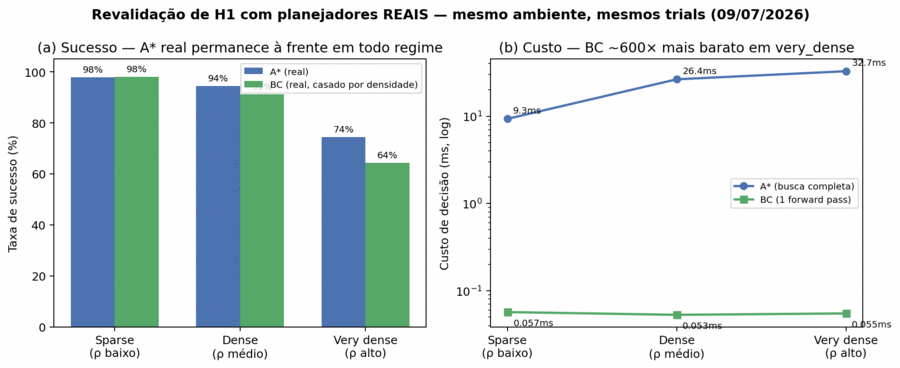
\includegraphics[width=0.68\textwidth]{figs/2d/fig_2d_h1_real_validation.png}
  \caption{(a)~Taxa de sucesso real, A* vs.\ BC casado por densidade: A* permanece à
           frente em todo regime. (b)~Custo de decisão real, escala logarítmica: BC
           $\sim$656$\times$ mais barato em \textit{very\_dense}. Dados reais, 1.500 trials
           pareados, \texttt{results\_abstract/h1\_real\_2d\_mixed\_pool.csv}.}
  \label{fig:h1_real_validation}
\end{figure}

Os valores acima são médias, e a distribuição completa acrescenta um detalhe relevante: o A*
apresenta cauda longa em \textit{very\_dense}, com \textit{outliers} de até 51,9~ms, enquanto a
variância do BC é desprezível. O contraste é o esperado entre uma busca em grafo e um único
\textit{forward pass}. Uma margem de segurança de 0,08~m além do raio do robô evita que o
controlador \textit{pure-pursuit} corte cantos: sem ela, a colisão chegava a 40\% em
\textit{very\_dense}, artefato do controlador e não do planejador; com ela, caiu para 0--9\%.

A substituição da linha reta pelo A* real também alcança o cenário multiagente, onde confirma que
nenhum planejador independente evita colisão entre robôs de forma confiável sem coordenação: o A*
real colide entre 65\% e 80\% das vezes conforme a densidade, com $N{=}4$, contra os 0\% que a
medição anterior, feita sobre a política de linha reta, alegava incorretamente.

A tese que sobrevive aos dados reais é mais modesta que a original. O $\rho$-criterion mantém
taxa de sucesso próxima à do melhor planejador fixo, o A*, por uma fração pequena do seu custo
computacional em alta densidade, com sucesso e custo medidos no mesmo ambiente e sobre os mesmos
trials.
\label{sec:urbano}

% ============================================================
\section{Conclusão}

As três hipóteses formuladas na Seção~1.1 foram endereçadas da seguinte forma.

H1 nasceu ambiciosa: ``a seleção adaptiva supera qualquer método fixo''. Os dados reais a
reformularam. A validação Monte Carlo (Seção~\ref{sec:validacao_fase1}) sustentava essa versão
sobre planejadores mock, mas a revalidação com A* e BC reais (Seção~\ref{sec:h1_real}) derrubou a
motivação por taxa de sucesso e reforçou a motivação por custo computacional. Sobra uma tese mais
modesta e sustentada por medição direta: o $\rho$-criterion mantém taxa de sucesso próxima à do
melhor planejador fixo por uma fração pequena do seu custo computacional em alta densidade.

Quanto à qualidade da fronteira de decisão, H2 se confirma. O $\rho$-criterion perde em média
2,9\% para o VBS, com 6,7\% no pior caso, dentro do limite de 10\% estabelecido. O custo dá ao
limiar uma segunda justificativa: naquele ponto o tempo do A* cresce dez vezes, enquanto a
latência da política aprendida não se move.

H3 também se confirma. A infraestrutura completa foi implantada em ROS2 Humble, Gazebo Classic e
TurtleBot3 Waffle sem exigir modificação dos planejadores subjacentes, uma contribuição de
engenharia replicável em qualquer \textit{stack} ROS2 + SB3 + Gazebo Classic.

Fica como contribuição central o $\rho$-criterion com limiar $\rho^*{=}0{,}30$: um critério de
seleção adaptiva independente dos planejadores subjacentes, aplicável a qualquer par formado por
um planejador clássico e uma política aprendida, em domínios onde a densidade local de obstáculos
seja estimável em tempo real a partir do LIDAR.

\textbf{Cobertura dos objetivos do Plano de Trabalho (PI08078-2024).} Dos cinco objetivos
específicos, três foram cumpridos integralmente e dois parcialmente. Cumpridos: (1)~implementação
dos algoritmos clássicos, com estruturas de dados otimizadas e benchmark real de tempo e memória
(Seção~\ref{sec:benchmark_classicos}, Tabela~\ref{tab:tempo_memoria}); (3)~identificação e teste
de abordagens de aprendizado por reforço profundo, com SAC como método principal, CrossQ testado
e descartado por baixo desempenho, e DDPG substituído por SAC sem teste isolado (ver
Limitações); e (4)~comparação entre métodos clássicos e modernos em tempo de execução e
eficiência computacional (Tabela~\ref{tab:tempo_memoria} e Seção~\ref{sec:h1_real}, incluindo o
custo do próprio critério adaptativo). Parcialmente cumpridos: (2)~avaliação em cenários
estáticos, dinâmicos e com obstáculos, o estático coberto na Fase~1
(Seção~\ref{sec:validacao_fase1}) e o dinâmico no gêmeo 2D (Seção~\ref{sec:h1_real}, obstáculo
móvel programado), mas não no Gazebo real, por falta de atores móveis nativos no Gazebo Classic;
e (5)~uso de Python, C++, ROS e Gazebo, Python e C++ (via Nav2/SmacPlanner2D) plenamente
empregados, Gazebo com infraestrutura completa mas sem validação quantitativa de navegação (ver
Limitação~1).

\textbf{Limitações.} (1)~A validação quantitativa com planejadores reais em Gazebo não foi
concluída nesta IC. O protocolo planejado ($N{=}30$ trials/condição, 3 seeds, Wilcoxon com
correção Holm-Bonferroni) foi implementado, mas não produziu dados válidos no prazo: a janela de
física despausada a cada passo de controle mostrou-se curta demais para o robô ganhar
velocidade sob o \texttt{max\_wheel\_acceleration} do TurtleBot3, que permanece parado mesmo com
o comando correto publicado, confirmado pela comparação entre um comando manual sustentado, que
move o robô normalmente, e o ciclo \texttt{step()} real da pipeline, com deslocamento próximo de
zero. O diagnóstico está registrado para retomada futura. (2)~O critério usa contexto
unidimensional e limiar fixo offline, por restrição de tempo real; contexto vetorial,
meta-aprendizado online e fusão suave são extensões naturais para cenários onde essa restrição
for menos severa. (3)~A avaliação restringiu-se ao TurtleBot3 Waffle em Gazebo Classic, sem
generalização testada a outras cinemáticas ou simuladores; e o SAC, treinado apenas no mundo
esparso, generaliza mal fora dele (91\% para 40\% de sucesso, Figura~\ref{fig:ic_degradation}),
motivando um currículo multi-densidade como próximo passo.

O trabalho progride em três fases: agente único (Fase~1), multi-agente via CBS (Fase~2,
parcial) e MARL (Fase~3, futuro).

% ============================================================
\renewcommand{\refname}{}
\section*{Referências Bibliográficas}
\addcontentsline{toc}{section}{Referências Bibliográficas}

\begin{thebibliography}{99}
\setlength{\itemsep}{6pt}
\setlength{\parskip}{2pt}
\small

\bibitem{Cimurs2022}
CIMURS, R.; SUH, I. H.; LEE, J. H. Goal-driven autonomous exploration through deep
reinforcement learning. \textbf{IEEE Robotics and Automation Letters}, v.~7, n.~2,
p.~730--737, 2022. DOI: 10.1109/LRA.2021.3133591.

\bibitem{Cormen2022}
CORMEN, T. H. et al. \textbf{Introduction to Algorithms}. 4.\ ed. Cambridge: MIT Press, 2022.

\bibitem{Damanik2024}
DAMANIK, J. J.; JUNG, J.-W.; DERESA, C. A.; CHOI, H.-L. LiCS: navigation using
learned-imitation on cluttered space. \textbf{IEEE Robotics and Automation Letters}, 2024.
DOI: 10.1109/LRA.2024.3518078.

\bibitem{Dey2023}
DEY, S.; SADEK, A.; MONACI, G.; CHIDLOVSKII, B.; WOLF, C. Learning whom to trust in
navigation: dynamically switching between classical and neural planning. In:
\textbf{IEEE/RSJ International Conference on Intelligent Robots and Systems (IROS)}, p.~5235--5242,
2023. arXiv:2307.16710.

\bibitem{Haarnoja2018}
HAARNOJA, T. et al. Soft actor-critic: off-policy maximum entropy deep reinforcement learning
with a stochastic actor. In: \textbf{International Conference on Machine Learning (ICML)},
p.~1861--1870, 2018.

\bibitem{Hart1968}
HART, P. E.; NILSSON, N. J.; RAPHAEL, B. A formal basis for the heuristic determination of
minimum cost paths. \textbf{IEEE Transactions on Systems Science and Cybernetics}, v.~4,
n.~2, p.~100--107, 1968.

\bibitem{Hespanha2003}
HESPANHA, J. P.; LIBERZON, D.; MORSE, A. S. Hysteresis-based switching algorithms for
supervisory control of uncertain systems. \textbf{Automatica}, v.~39, p.~263--272, 2003.

\bibitem{Kolomeytsev2025}
KOLOMEYTSEV, Y.; GOLEMBIOVSKY, D. Hybrid motion planning with deep reinforcement learning
for mobile robot navigation. \textbf{arXiv preprint}, 2025. arXiv:2512.24651.

\bibitem{Macenski2022}
MACENSKI, S. et al. Robot operating system 2: design, architecture, and uses in the wild.
\textbf{Science Robotics}, v.~7, n.~66, 2022.

\bibitem{Raffin2021}
RAFFIN, A. et al. Stable-baselines3: reliable reinforcement learning implementations.
\textbf{Journal of Machine Learning Research}, v.~22, n.~268, p.~1--8, 2021.

\bibitem{Rice1976}
RICE, J. R. The algorithm selection problem. \textbf{Advances in Computers}, v.~15,
p.~65--118, 1976.

\bibitem{Sharma2024}
SHARMA, V. D. et al. Hybrid classical/RL local planner for ground robot navigation.
\textbf{arXiv preprint}, 2024. arXiv:2410.03066.

\bibitem{Xu2020}
XU, Z.; DHAMANKAR, G.; NAIR, A.; XIAO, X.; WARNELL, G.; LIU, B.; WANG, Z.; STONE, P. APPLR:
adaptive planner parameter learning from reinforcement. \textbf{arXiv preprint}, 2020.
arXiv:2011.00397.

\bibitem{deJesus2021}
DE JESUS, J. C. et al. Soft actor-critic for navigation of mobile robots.
\textbf{Journal of Intelligent \& Robotic Systems}, v.~102, n.~2, 2021.
DOI: 10.1007/s10846-021-01367-5.

\end{thebibliography}

% ============================================================
\newpage
\section*{Informações Complementares}
\addcontentsline{toc}{section}{Informações Complementares}

\subsection*{Certificados: Diálogos em Pesquisa e Inovação}
Certificados anexados ao final deste documento (emitidos pela Pró-Reitoria de Pesquisa e
Inovação da UFG, autenticidade verificável nas URLs impressas em cada certificado):
\begin{itemize}\setlength{\itemsep}{0pt}\setlength{\parskip}{0pt}
  \item ``Currículo Lattes: dicas de preenchimento e atualização'' (27/03/2026, 2h).
  \item 22º CONPEEX, participação como ouvinte (04--07/11/2025, 40h).
  \item Palestra ``Ciência no Calor do Cerrado'', no 22º CONPEEX (05/11/2025, 4h).
  \item ``Estratégias e boas práticas para apresentação de trabalhos científicos''
        (13/08/2026, 2h).
\end{itemize}


\includepdf[pages=-,fitpaper=true]{certificados/certificado_curriculo_lattes.pdf}
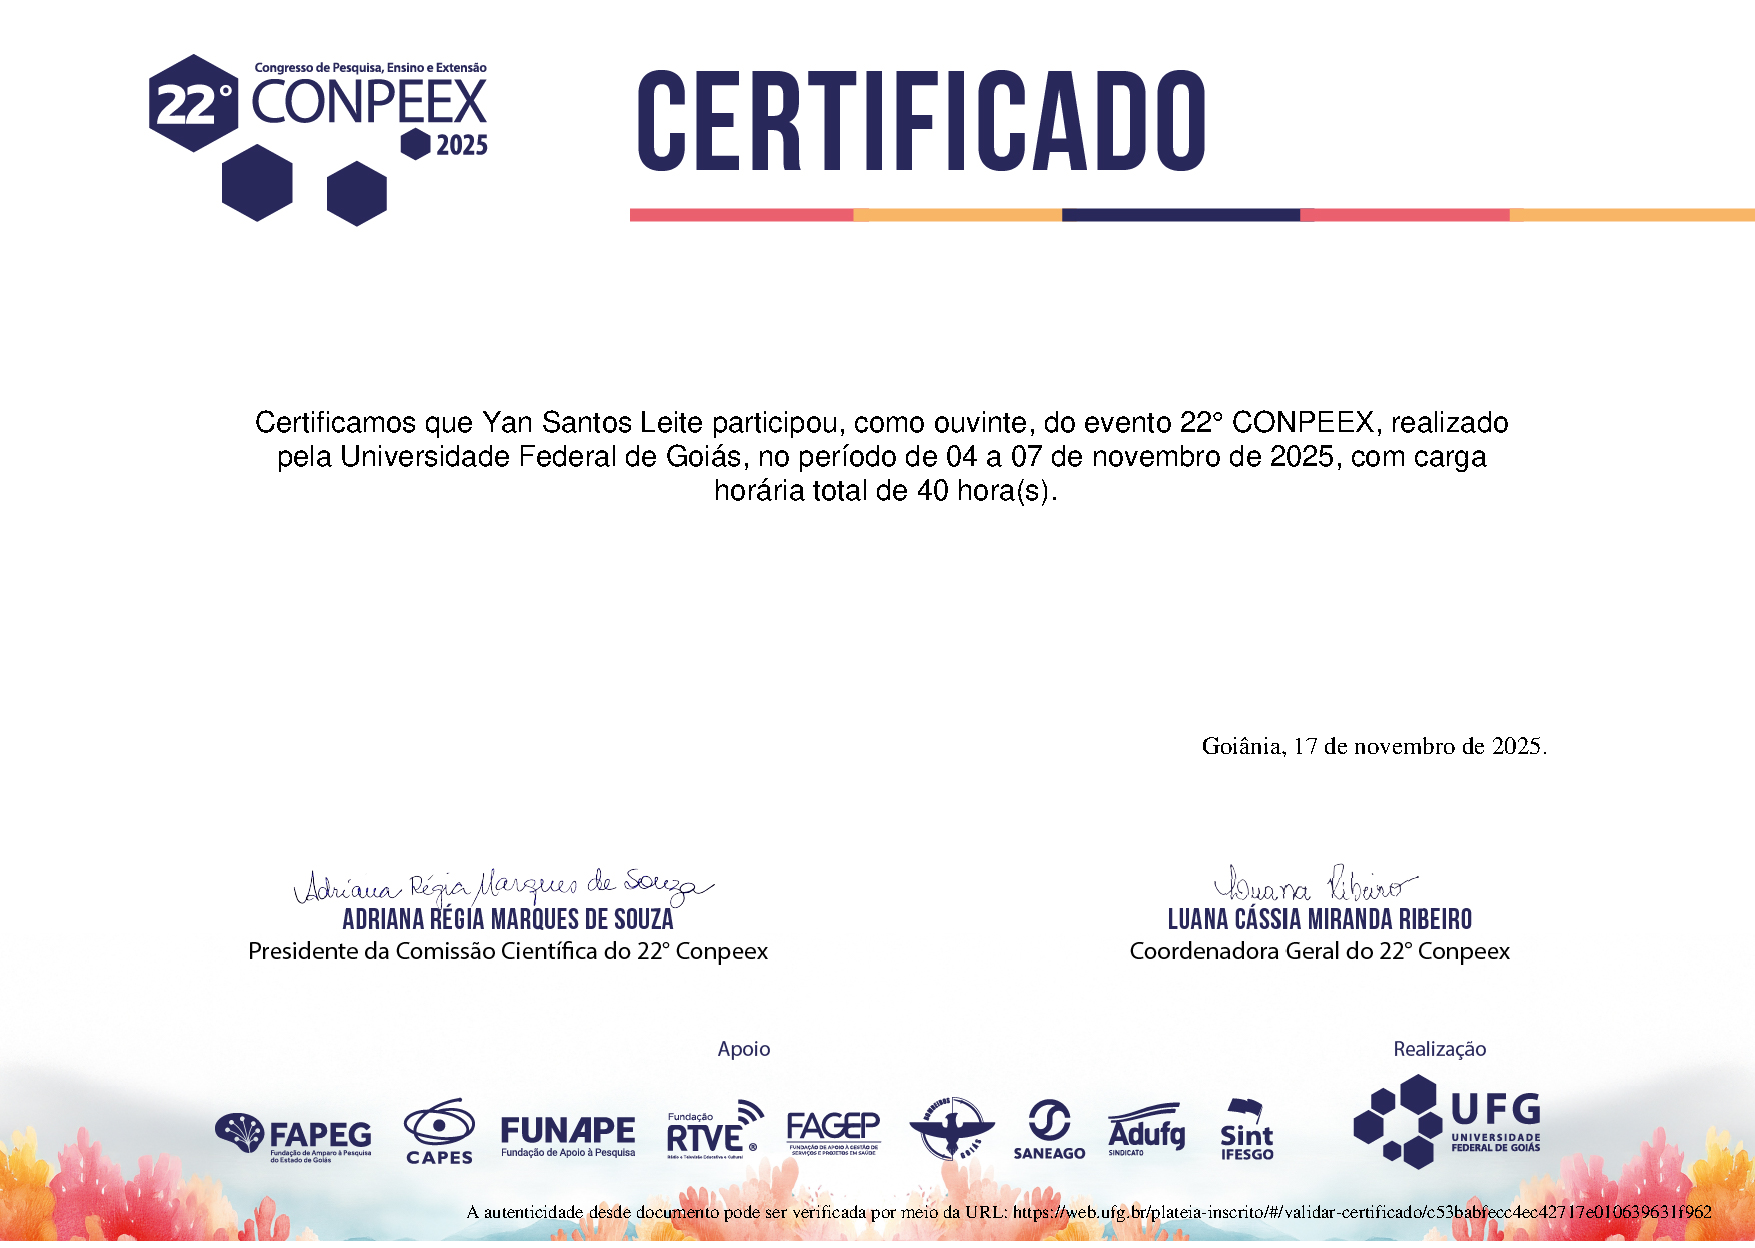
\includepdf[pages=-,fitpaper=true]{certificados/certificado_conpeex.pdf}

\includepdf[pages=-,fitpaper=true]{certificados/certificado_ciencia_calor_cerrado.pdf}

\includepdf[pages=-,fitpaper=true]{certificados/certificado_estrategias_apresentacao.pdf}

\end{document}
